%% Implementation Phase Presentation Template (KIT Beamer)
\documentclass{sdqbeamer}[en]
\usepackage{booktabs}
\usepackage{amssymb}

\grouplogo{codex_logo} 
\groupname{ITEC - Institute of Computer Engineering}

\title[Implementation Phase]{CodeX: Natural Language to Structured Code Generation}
\subtitle{Implementation Phase} 
\author[Oleksandr Brittner]{\textbf{Oleksandr Brittner}, Simon Bumiller, Simon Gaber, Dayana Karadzhova, Kyrylo Pavlov \newline}
\date[6.\,03.\,2026]{March 6, 2026}

\usepackage{lipsum}
\usepackage{pdfpages}
\usepackage{listings}
\usepackage{pifont}

\newcommand{\cmark}{\ding{51}} % checkmark
\newcommand{\xmark}{\ding{55}} % cross
\newcommand{\omark}{\ding{108}} % circle

\begin{document}

% Titelseite
\begin{frame}[title green horizontal, picture=images/programming-languages, kitlogo=white]
\titlepage
\end{frame}

% Inhaltsverzeichnis
\begin{frame}[tableofcontents=green]{Content}
\tableofcontents
\end{frame}

\section{General Overview}
\begin{frame}[t]{General Overview}{Development Schedule}

\centering
\only<1->{
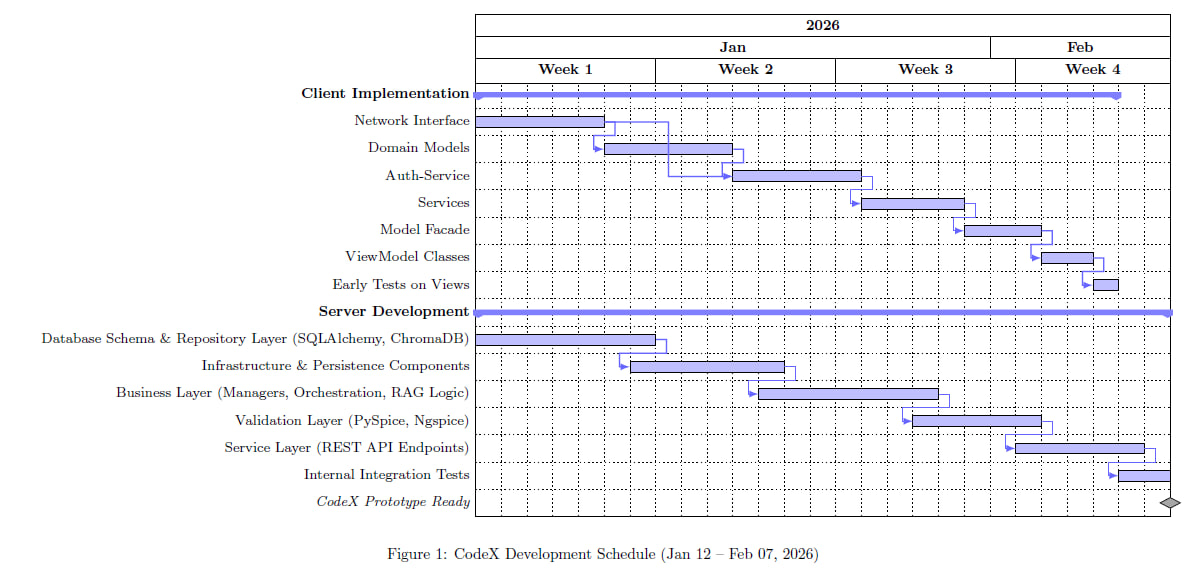
\includegraphics[scale=0.8]{images/gannt_planned.jpg}
}

\end{frame}

\begin{frame}[t]{General Overview}{Client}

\centering
\only<1->{
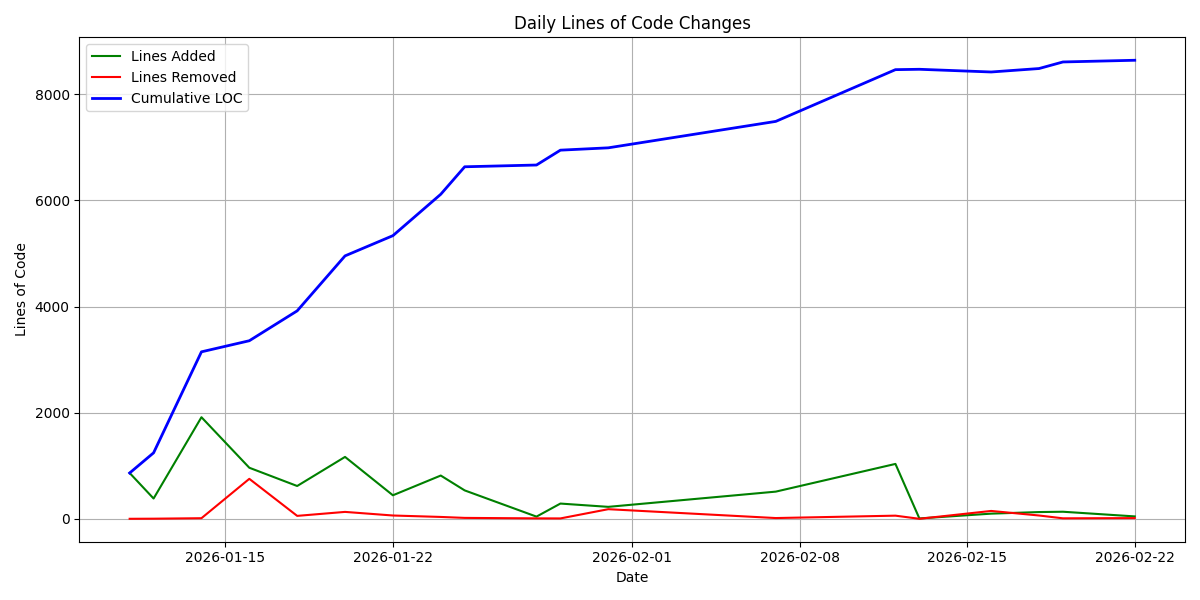
\includegraphics[scale=0.8]{images/client_loc.png}
}

\end{frame}

\begin{frame}[t]{General Overview}{Server}


\centering
\only<1->{
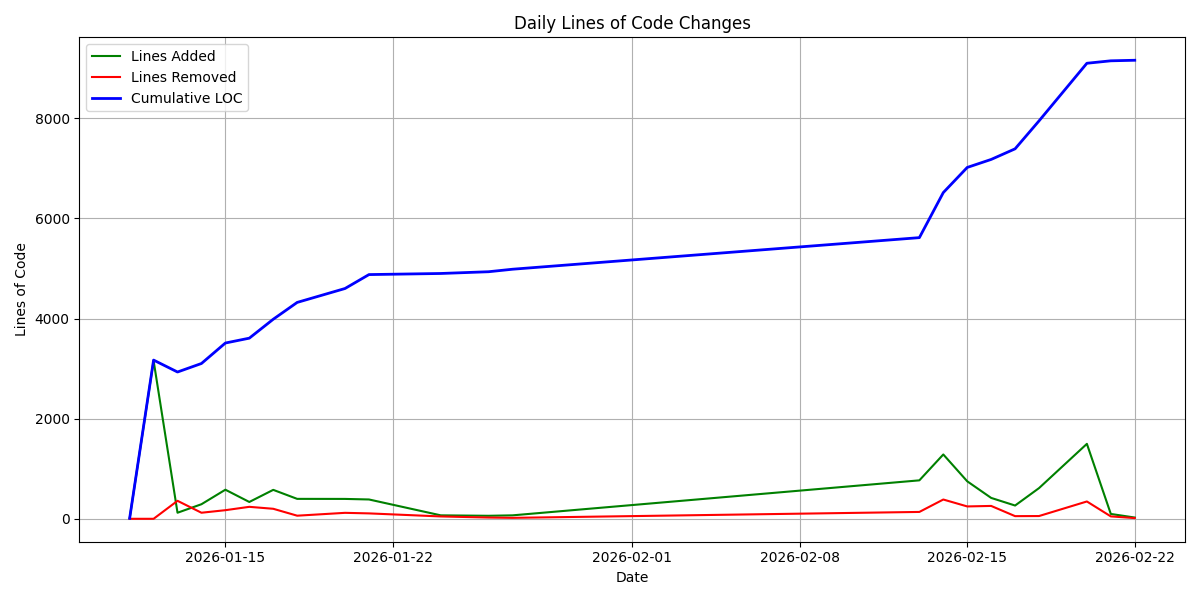
\includegraphics[scale=0.8]{images/server_loc.png}
}

\end{frame}

%% ------------------------
\section{Stand of Implementation}

\begin{frame}[t]{Stand of Implementation}{Must Criteria}

\begin{tabular}{p{0.1\textwidth} p{0.75\textwidth} c}

\only<1->{\textbf{RM1} & The system must provide a web interface that allows natural language to be converted into a snippet of code. The target DSL can be selected from available options and the generated code can be exported as a file. & \cmark \\}

\only<2->{\textbf{RM2} & The system must provide SPICE as one option of its selectable DSLs. & \cmark \\}

\only<3->{\textbf{RM3} & SPICE conversations must include a visualization of the respective circuit. & \cmark \\}

\only<4->{\textbf{RM4} & Every conversation must have a name. & \cmark \\}

\only<5->{\textbf{RM5} & The system must support LLM requests using a Retrieval-Augmented Generation (RAG) approach. Retrieved data must be stored in a secure database that respects intellectual property constraints. & \cmark \\}

\only<6->{\textbf{RM6} & The system must integrate a validation back-end to validate the generated circuit for SPICE conversations. & \cmark \\}

\only<7->{\textbf{RM7} & The system must allow adding and removing separate LLM models together with their OpenAI API URL. When a request is made, the user must be able to select the model with which the request will be performed. & \cmark \\}

\end{tabular}

\end{frame}

\begin{frame}[t]{Stand of Implementation}{Should Criteria}

\begin{tabular}{p{0.1\textwidth} p{0.75\textwidth} c}

\only<1->{\textbf{RS1} & The circuit visualization for SPICE should be interactive. & \cmark \\}

\only<2->{\textbf{RS2} & The interface of the system should allow users to cancel a pending request. & \xmark \\}

\only<3->{\textbf{RS3} & Users should be able to sign up, log in, and log out using a username (or email) and password. & \cmark \\}

\only<4->{\textbf{RS4} & A strict password complexity policy should be implemented. & \omark \\}

\only<5->{\textbf{RS5} & The system should allow users to securely update their profile data. & \cmark \\}

\only<6->{\textbf{RS6} & The system should provide a secure mechanism for users to recover their accounts in case of lost credentials. & \cmark \\}

\only<7->{\textbf{RS7} & Conversations should be stored with respect to the account that created them and be visible only to that account. & \cmark \\}

\only<8->{\textbf{RS8} & If the LLM fails to generate working code after multiple retries, the system should stop further attempts and display an appropriate error message indicating the failure. & \cmark \\}

\only<9->{\textbf{RS9} & The system should provide a list of all previous conversations and allow users to view them. & \cmark \\}

\only<10->{\textbf{RS10} & Every conversation should be able to be marked as deleted and should not be shown in the overview afterwards. & \cmark \\}

\end{tabular}

\end{frame}
\begin{frame}[t]{Stand of Implementation}{Could Criteria (1/2)}

\begin{tabular}{p{0.1\textwidth} p{0.75\textwidth} c}

\onslide<1->{\textbf{RC1} & The system could integrate a simulation back-end to simulate the generated circuit for SPICE conversations. & \cmark \\}

\onslide<2->{\textbf{RC2} & The system could accept follow-up instructions on conversations. & \cmark \\}

\onslide<3->{\textbf{RC3} & The system could provide more DSL options than only SPICE. & \cmark \\}

\onslide<4->{\textbf{RC4} & Every account could be associated with the role Admin or Member. Each role could have a configurable upper bound of requests per month set as a server parameter. & \cmark \\}

\onslide<5->{\textbf{RC5} & The role request upper bounds could be configured by administrators via the web interface. & \cmark \\}

\onslide<6->{\textbf{RC6} & The web interface could be offered in multiple languages, at least German and English. & \cmark \\}

\onslide<7->{\textbf{RC7} & If supported by the DSL, the generated code output could be prettified using syntax highlighting. & \xmark \\}

\onslide<8->{\textbf{RC8} & The front-end could allow users to pin a conversation so that it remains at the top of the conversation list. & \cmark \\}

\end{tabular}

\end{frame}

\begin{frame}[t]{Stand of Implementation}{Could Criteria (2/2)}

\begin{tabular}{p{0.1\textwidth} p{0.75\textwidth} c}

\onslide<1->{\textbf{RC9} & During registration, the user’s email could be confirmed via a verification link or code. Registration would not be completed until confirmation. Changing the email would automatically trigger a new confirmation. & \cmark \\}

\onslide<2->{\textbf{RC10} & The system could support OAuth 2.0 authentication to allow login via trusted providers such as Google. & \cmark \\}

\onslide<3->{\textbf{RC11} & The software could provide a dark mode as an alternative theme. & \cmark \\}

\onslide<4->{\textbf{RC12} & The system could integrate with cloud storage providers to save or share generated code snippets. & \xmark \\}

\onslide<5->{\textbf{RC13} & The application could allow users to search conversations by name. & \cmark \\}

\onslide<6->{\textbf{RC14} & The front-end could indicate to the user that a request is currently being processed. & \cmark \\}

\onslide<7->{\textbf{RC15} & The software could allow users to download generated code as a file. & \cmark \\}

\onslide<8->{\textbf{RC16} & The software could provide admin-only analytics on usage (e.g., daily active users) not visible to regular users. & \xmark \\}

\onslide<9->{\textbf{RC17} & Users could upload and display a profile picture associated with their account. & \cmark \\}

\end{tabular}

\end{frame}

%% ------------------------
\section{Working Methods}

\begin{frame}[t]{Working Methods}{Internal Communication}

\onslide<1->{\textbf{Communication Strategy}}

\begin{itemize}
\onslide<1->{\item Effective communication was essential for coordinating development tasks and resolving technical challenges.}
\onslide<1->{\item The team combined digital communication tools with regular in-person meetings.}
\end{itemize}

\vspace{0.5em}

\onslide<2->{\textbf{Digital Communication}}

\begin{itemize}
\onslide<2->{\item \textbf{WhatsApp:} Used for quick coordination, status updates, and short questions during daily work.}
\onslide<2->{\item \textbf{Discord:} Used for more technical discussions, design decisions, and collaborative problem solving.}
\end{itemize}

\vspace{0.5em}

\onslide<3->{\textbf{In-Person Meetings}}

\begin{itemize}
\onslide<3->{\item Regular on-site meetings were held to review progress and plan upcoming tasks.}
\onslide<3->{\item Face-to-face discussions helped resolve complex issues and align the team on architectural decisions.}
\end{itemize}

\vspace{0.5em}

\onslide<4->{\textbf{Outcome}}

\begin{itemize}
\onslide<4->{\item Clear task responsibilities and documented decisions.}
\onslide<4->{\item Efficient coordination and quick resolution of misunderstandings.}
\end{itemize}

\end{frame}

\begin{frame}[t]{Working Methods}{Version Control}

\centering
\onslide<1->{
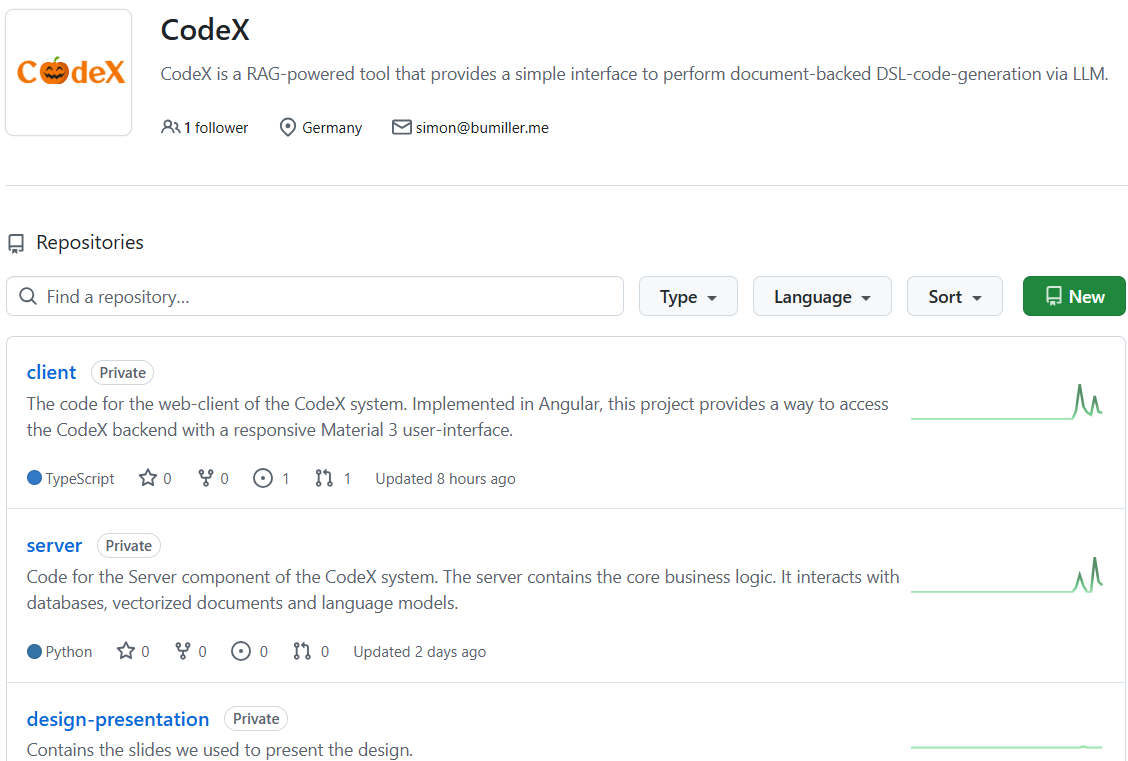
\includegraphics[scale=0.7]{images/git-photo.png}
}

\end{frame}

\begin{frame}[t]{Working Methods}{IDEs}

\textbf{Integrated Development Environments}

\begin{itemize}
\onslide<1->{\item Developers were free to choose tools based on personal preference and workflow.}
\end{itemize}

\vspace{0.5em}

\onslide<2->{\textbf{IDEs used in the project}}

\begin{itemize}
\onslide<2->{\item JetBrains PyCharm}
\onslide<2->{\item JetBrains WebStorm}
\onslide<2->{\item Visual Studio Code}
\end{itemize}

\end{frame}
\begin{frame}[t]{Environment}{Components and Tools}

\onslide<1->{\textbf{System Components}}

\begin{itemize}
\onslide<1->{\item \textbf{Client:} Angular-based web interface}
\onslide<1->{\item \textbf{Server:} FastAPI backend providing REST API}
\onslide<1->{\item \textbf{Database:} PostgreSQL for persistent data storage}
\onslide<1->{\item \textbf{Vector Database:} ChromaDB for retrieval in the RAG pipeline}
\end{itemize}

\vspace{0.5em}

\onslide<2->{\textbf{Infrastructure and Tools}}

\begin{itemize}
\onslide<2->{\item \textbf{Version Control:} Git with GitHub repositories}
\onslide<2->{\item \textbf{Branching Workflow:} Feature and layer-based branches}
\onslide<2->{\item \textbf{Containerization:} Docker images for client and server}
\onslide<2->{\item \textbf{Deployment:} Docker Compose orchestrating services}
\end{itemize}

\vspace{0.5em}

\onslide<3->{\textbf{External Interfaces}}

\begin{itemize}
\onslide<3->{\item OpenAI-compatible model APIs}
\onslide<3->{\item Authentication providers (OAuth / Google login)}
\end{itemize}

\end{frame}

%% ------------------------
\section{Implementation Highlights}



\begin{frame}[t]{Key Features}{User Interface}

\textbf{Navigation and Conversation Management}

\begin{itemize}
    \item Clean web interface for interacting with the system.
    \item Sidebar navigation listing all user conversations.
    \item Conversations can be created, opened, or removed.
\end{itemize}

\vspace{0.4cm}

\textbf{Conversation Screen}

\begin{itemize}
    \item Chat-like interface for natural language prompts.
    \item Generated DSL code displayed directly in the conversation.
    \item SPICE circuits automatically visualized.
    \item Generated code can be exported as a file.
\end{itemize}

\end{frame}


\begin{frame}[t]{Key Features}{Authentication and Admin Panel}

\onslide<1->{
\textbf{User Authentication}

\begin{itemize}
    \item Secure user registration and login.
    \item Password-based authentication with encrypted storage.
    \item Optional OAuth login using external providers.
\end{itemize}
}

\vspace{0.4cm}

\onslide<2->{
\textbf{User Management}

\begin{itemize}
    \item Each user has a personal set of conversations.
    \item Conversations are accessible only to their creator.
\end{itemize}
}

\vspace{0.4cm}

\onslide<3->{
\textbf{Admin Panel}

\begin{itemize}
    \item Admin users can manage system configuration.
    \item Control usage limits and system parameters.
    \item Monitor system usage and manage models.
\end{itemize}
}

\end{frame}
\begin{frame}[t]{Key Features}{Settings and Configurations}

\onslide<1->{
\textbf{LLM Configuration}

\begin{itemize}
    \item Support for multiple Large Language Models.
    \item Configurable API endpoints for external model providers.
    \item Users can select the model used for code generation.
\end{itemize}
}

\vspace{0.4cm}

\onslide<2->{
\textbf{User Settings}

\begin{itemize}
    \item Profile management and account settings.
    \item Language preferences and interface customization.
    \item Personal conversation history and organization.
\end{itemize}
}

\vspace{0.4cm}

\onslide<3->{
\textbf{System Flexibility}

\begin{itemize}
    \item New models can be added or removed dynamically.
    \item Configuration handled through the web interface.
\end{itemize}
}

\end{frame}


\begin{frame}[t]{Core Functionality}{RAG, SPICE Generation, Visualization}

\onslide<1->{
\textbf{Retrieval-Augmented Generation (RAG)}

\begin{itemize}
    \item User prompt is enriched with relevant retrieved knowledge.
    \item Vector database used to store and retrieve documentation.
    \item Improves accuracy and reliability of generated code.
\end{itemize}
}

\vspace{0.4cm}

\onslide<2->{
\textbf{SPICE Code Generation}

\begin{itemize}
    \item Natural language instructions translated into SPICE circuits.
    \item Generated code validated by a dedicated validation backend.
\end{itemize}
}

\vspace{0.4cm}

\onslide<3->{
\textbf{Circuit Visualization}

\begin{itemize}
    \item Generated SPICE circuits rendered visually.
    \item Interactive visualization allows users to inspect circuit structure.
\end{itemize}
}

\end{frame}
%% ------------------------
\section{Challenges \& Solutions}

\begin{frame}[t]{Challenges}{Technical and Implementation Obstacles}

\onslide<1->{
\textbf{Learning Curve}

\begin{itemize}
    \item New technologies such as FastAPI, Angular, and asynchronous request handling required additional learning time.
\end{itemize}
}

\vspace{0.4cm}

\onslide<2->{
\textbf{System Integration}

\begin{itemize}
    \item Integrating multiple components: client, backend, databases, and external LLM APIs.
\end{itemize}
}

\vspace{0.4cm}

\onslide<3->{
\textbf{Architecture Adjustments}

\begin{itemize}
    \item Initial architectural assumptions required revisions during development.
    \item Refactoring was necessary to maintain modularity and scalability.
\end{itemize}
}

\vspace{0.4cm}

\onslide<4->{
\textbf{Time Constraints}

\begin{itemize}
    \item Some optional features and extended testing had to be deprioritized to meet deadlines.
\end{itemize}
}

\end{frame}

\begin{frame}[t]{Solutions}{How Challenges Were Addressed}

\onslide<1->{
\textbf{Incremental Development}

\begin{itemize}
    \item Components were developed in parallel once stable interfaces were defined.
\end{itemize}
}

\vspace{0.4cm}

\onslide<2->{
\textbf{Collaboration and Communication}

\begin{itemize}
    \item Regular meetings and active team communication enabled quick issue resolution.
\end{itemize}
}

\vspace{0.4cm}

\onslide<3->{
\textbf{Feature Prioritization}

\begin{itemize}
    \item Focus placed on implementing all core requirements first.
    \item Optional features were postponed when necessary.
\end{itemize}
}

\end{frame}

\begin{frame}[c]{Demo \& Conclusion}

\begin{center}

\onslide<1->{\Large Now we will demonstrate our CodeX web application.}\\[0.6cm]

\onslide<1->{\Large Thank you for your attention!}

\end{center}

\end{frame}

%% ------------------------

\end{document}